\documentclass[11pt]{article}
\usepackage{graphicx}
\usepackage{lipsum}
\begin{document}

\begin{titlepage}

\begin{center}
\begin{huge}
Swarm Visualiser - COS 301 Main Project
\\
Testing Specifications
\begin{small}
\\
Team: Dragon Brain
\\
Members:
\\
Matheu Botha u14284104
\\
Renton McInytre u14312710
\\
Emilio Singh u14006512
\\
Gerard van Wyk u14101263

\end{small}

\end{huge}
\end{center}
\end{titlepage}

\pagebreak

\tableofcontents

\pagebreak
\section{Introduction}
\subsection{Purpose}
This document describes the testing methodologies and frameworks used in the Swarm Visualiser project by team DragonBrain. The general purpose of the project is to create a functional experimental and teaching tool that allows the functioning of a Particle Swarm Optimisation problem solver to be conceptualised and visualised to display a more comprehensible impression of the inner workings of such systems.
\newline This document serves as a recording of the methods and specific tests used to ensure proper functionality of the project, thus permitting proper test driven development processes to be followed. This is a necessity in order to ensure that the system in question has minimal risk of failure as the system develops.


\subsection{Scope}
This document is structured as follows:
\begin{itemize}
    \item Tests that have been identified are specified in section 2.
    \item Features to be tested are specified in section 3.
    \item Sections 4 through 6 will discuss the tests indepth.
    \item Section 7 will discuss the results of the testing.
    \item Sections 8 and 9 will conclude with additional comments and explanations.
    \item The remainder of this section will be used to discuss the testing environment, as well as assumptions and dependencies.
\end{itemize}

\subsection{Test Environment}
The environment of the testing system is as follows:
\begin{itemize}
    \item Programming Languages: C++ has been used as the base language with which the system is coded. Additionally, graphical subsections of the system make use of OpenGL and the Graphical User Interface is made using Qt libraries.
    \item Testing Frameworks: The system's unit tests are run and handled using the cross-platform Unit Testing library, Google Test, Google's own testing framework for C++ applications.
    \item Coding Environment: All coding has been done using CLion, Jetbrains' IDE for C++ (which has integrated support for Google Tests), along with CMake for automated building of the system.
    \item Operating System: In true spirit of cross-compatibility, tests have been run under two particular operating systems, namely Windows 10 and Linux Mint (a distribution of Linux).
\end{itemize}

\subsection{Assumptions and Dependencies}
For the sake of these tests, the following dependencies between subsystems are assumed:
\begin{itemize}
    \item The Manager depends upon the Settings Package, the Graphics Pipeline, the General Optimiser and the Snapshot Manager.
    \item The Graphics Pipeline depends on the Snapshot Manager and the Settings Package.
    \item The General Optimiser depends on the Snapshot Manager and the Settings Package.
\end{itemize}


\section{Test Items}
Following is a list of the unit tests performed:
\begin{itemize}
    \item Snapshot Manager subsystem functionality.
    \item General Optimiser subsystem functionality.
    \item Settings Package subsystem functionality.
\end{itemize}

\section{Functional Features to be Tested}
\subsection{Snapshot Manager}
The features to be tested are as follows:
\begin{itemize}
    \item The ability of the subsystem to create a correct snapshot of the current particle situation.
    \item The ability of the subsystem to correctly function as a standard queue of snapshots (hence, the ability to enqueue and dequeue snapshots correctly).
    \item The ability of the subsystem to handle additional bounded queue functionality.
\end{itemize}
These are all low level tests that will be tested with a series of simple assertion-like methods, to ensure that the queue functions as it is meant to. The queue's main design requirement is Scalability.

\subsection{General Optimiser}
The features to be tested are as follows:
\begin{itemize}
    \item The ability of the subsystem to correctly generate particle objects.
    \item The ability of the subsystem to correctly generate a swarm with a valid n-matrix.
\end{itemize}


\subsection{Settings Package}
The features to be tested are as follows:
\begin{itemize}
    \item The ability of the subsystem to create a valid Graphics Settings Package.
    \item The ability of the subsystem to create a valid Problem Domain Settings Package.
    \item The ability of the subsystem to create a valid Optimiser Settings Package.
\end{itemize}

\section{Test Cases}
\subsection{Snapshot Manager}
\subsubsection{Case 1: Generating a Snapshot}
\begin{itemize}
    \item Objective: To ensure basic generation of a Snapshot is functional.
    \item Input: An array of Particles and an array of integers representing the links between them.
    \item To assume a pass result, the expected outcome is for a single Snapshot which has the Particles and links as members to be created.
\end{itemize}

\subsubsection{Case 2: Generating a Snapshot Queue}
\begin{itemize}
    \item Objective: To ensure basic generation of a Snapshot is functional.
    \item Input: An array of Particles and an array of integers representing the links between them.
    \item To assume a pass result, the expected outcome is for a single Snapshot which has the Particles and links as members to be created, which is then expected to be enqueued into the Snapshot Manager and dequeued successfully.
\end{itemize}

\subsection{General Optimiser}
\subsubsection{Case 1: Hill-climber OPT Process}
\begin{itemize}
    \item Objective: To ensure that during a single iteration, using the Hill-Climber process,that the particles are able to perform an optimisation action.  
    \item Input: \begin{itemize}
    \item A Snapshot consisting of the following:
    	\begin{itemize}
    	\item A particle Swarm
    	\item An Objective Function
    	\end{itemize}
    \end{itemize}
    \item To assume a pass result, the expected outcome is for at least one particle in the swarm to be at a position better than it originally was. In ideal conditions, the swarm would have every particle reach a better position, the best, and reach a convergence point but for the purposes of testing, at least one particle needs to be in a position better as defined by its objective function.
\end{itemize}
\subsubsection{Case 2: Conical PSO OPT Process}
\begin{itemize}
    \item Objective: To ensure that during a single iteration, using the Conical Particle Swarm Optimisation process,that the particles are able to perform an optimisation action.
    \item Input: \begin{itemize}
    \item A Snapshot consisting of the following:
    	\begin{itemize}
    	\item A particle Swarm
    	\item An Objective Function
    	\end{itemize}
    \end{itemize}
    \item To assume a pass result, the expected outcome is for at least one particle in the swarm to be at a position better than it originally was. In ideal conditions, the swarm would have every particle reach a better position, the best, and reach a convergence point but for the purposes of testing, at least one particle needs to be in a position better as defined by its objective function.
\end{itemize}
\subsubsection{Case 3: General PSO OPT Process}
\begin{itemize}
    \item Objective: To ensure that during a single iteration, using the general particle swarm optimisation process,that the particles are able to perform an optimisation action.
    \item Input: \begin{itemize}
    \item A Snapshot consisting of the following:
    	\begin{itemize}
    	\item A particle Swarm
    	\item An Objective Function
    	\end{itemize}
    \end{itemize}
    \item To assume a pass result, the expected outcome is for at least one particle in the swarm to be at a position better than it originally was. In ideal conditions, the swarm would have every particle reach a better position, the best, and reach a convergence point but for the purposes of testing, at least one particle needs to be in a position better as defined by its objective function.
\end{itemize}
\subsection{Settings Package}
\subsection{Case 1: Generatng a SettingsPackage Object}
\begin{itemize}
    \item Objective: To instantiate a SettingsPackage Object comprised of A ProblemDomainSettingsPackage, GraphicsSettingsPackage, and an OptimizerSettingsPackage, as well as some local independent variables.
    \item Input: A series of values for initialization of the various components
    \item: To assume a pass result, it must be confirmed that all composing objects of the SettingsPackage Object contain the attributes that are expected.
    \end{itemize}
\subsection{Objective functions}
\subsection{Case 1: Generating a sinObjective}
\begin{itemize}
    \item Objective: To instantiate a specific objective function(sinObjective) and test that it returns a value in the correct range, for a given random input.
    \item Function: sinObjective calculates the formula sin(x)+sin(y), where x and y are the 2 input parameters.
    \item Input:\begin{itemize}
        \item a sinObjective instance does not require any parameters for its constructor.
        \item the function in sinObjective is called with random parameters to assure that it is tested with a diversity of values, making the test more robust.
        \end{itemize}
    \item To achieve a pass result the value returned by sinObjective(after being called with random parameters) should always be within the range [0,2], if the returned value is outside of that range it is a fail result.
\end{itemize}
\subsection{Case 2: Checking the integrity of the AckleyObjective}
\begin{itemize}
	\item Objective: Determine if the Ackley Objective function is functioning as expected.
	\item Function:
	$$f(x_0 \cdots x_n) = -20 exp(-0.2 \sqrt{\frac{1}{n} \sum_{i=1}^n x_i^2}) - exp(\frac{1}{n} \sum_{i=1}^n cos(2\pi x_i)) + 20 + e$$ 
	
	$$-32 \leq x_i \leq 32$$ 
	\begin{center}
	\begin{verbatim}
	minimum at f(0, ... ,0) =0
	\end{verbatim}
	
	\end{center}
	
	
	\item Input: \begin{itemize}
		\item An AckleyObjective instance does not require any parameters for its constructor.
		\item The function in AckleyObjective is called with the specific value of (0,0) and then with a random value at any point other than (0,0).
	\end{itemize}
	\item If the function returns 0 for (0,0) and any positive value for the randomly chosen point, then it passes, otherwise it fails.
\end{itemize}

\subsection{Particle}
\subsubsection{setVelocity}
\begin{itemize}
	\item Objective: To ensure that a particle's velocity value can be set by being passed an external vector.
	\item Input: An array consisting of double values of a pre-specified length.
	\item To assume a pass result, the expected outcome is for the private array representing the particle's position vector to be set to exactly the values specified by the passed in array.
\end{itemize}
\subsubsection{setPositionAtDimension}
\begin{itemize}
	\item Objective: To ensure that a particle's position vector at a specific dimension can be set by being passed an external value.
	\item Input: Two double values: one representing the position value, the other the dimension.
	\item To assume a pass result, the expected outcome is for the private array at the specified dimension, representing the particle's position vector,  to be set to exactly the value specified by the parameter passed in.
		\end{itemize}
\subsubsection{getVelocity}
\begin{itemize}
	\item Objective: To ensure that a particle's velocity value can be set by being passed an external vector.
	\item Input: No input.
	\item To assume a pass result, the value returned must be the same as the value stored by the particle that getVelocity was called on.
\end{itemize}
\subsection{Graphics Processor}
\subsubsection{Case 1: Generating a Graphics Processor}
\begin{itemize}
	\item Objective: Ensure that a Graphics Processor is correctly instantiated with an objective function and a snapshot manager.
	\item Input: An objective function representing some mathematical formula.
	\item To assume a pass result, the expected outcome is for the graphics processor to correctly create a mesh from the given objective function as well as be able to dequeue from the snapshot manager and create a particle system from the snapshot.
\end{itemize}

\subsubsection{Case 2: Generating a Landscape Mesh}
\begin{itemize}
	\item Objective: Ensure that a mesh can be generated from a objective function.
	\item Input: An objective function representing some mathematical formula.
	\item To assume a pass result, it is expected that the given objective function will produce values from given co ordinates and create an accurate mesh that can be drawn to the screen.
\end{itemize}

\subsubsection{Case 3: Generating a particle System}
\begin{itemize}
	\item Objective: Ensure that a particle system can be generated from the snapshot manager.
	\item Input: A valid snapshot manager.
	\item To assume a pass result, it is expected that the graphics processor will be able to dequeue from the snapshot and use the particle co ordinates to create a particle system.s
\end{itemize}

\section{Item Pass/Fail Criteria}
Each item tested must meet criteria specific to its particular scenario in order to be considered passed or failed. These are tested with assertions and similar methodologies, hence if an item is failed it will be detected as such by Google Tests.

\subsection{General Optimiser: OPT Process}
\paragraph{•}
In general, the difficulty of testing is predicated on the stochastic nature of the particle system, exact precise testing is difficult. However, that being said, there are certain capacities that would be considered fail and considered a pass. 

\subparagraph{•}
The passing condition would require any combination of the following:
\begin{itemize}
\item At least one particle is in a better position according to the appropriate function.
\end{itemize}

\subparagraph{•}
The failing condition would require the following: 
\begin{itemize}
\item More than 50 percent of the particle swarm ended in a worse position than the previous iteration and it continues for at least some proportional(x) degree of the total number of iterations.
\end{itemize}


\section{Detailed Test Results}
\subsection{Snapshot Manager}
\subsubsection{Case 1: Generating a Snapshot}
The following results were obtained from the tests conducted. The tests to produce the
following results have \textbf{passed} and the reasons are stated below.

\begin{itemize}
	\item Created Snapshot Object and confirmed that the links are as they were expected to me.
	\item Snapshot Object has a list of particles matching the expectation.
\end{itemize}


\subsubsection{Case 2: Generating a Snapshot Queue}
The following results were obtained from the tests conducted. The tests to produce the
following results have passed and the reasons are stated below.

\begin{itemize}
	\item Basic Enqueue/Dequeue check passes (item enqueued correctly matches dequeued item).
	\item Bounded Queue behaviour demonstrated correctly (no further items enqueued after [bound] number of items have been enqueued).
	\item Dequeue fails correctly when attempting to dequeue from an empty queue.
\end{itemize}

\subsection{General Optimiser}
\subsubsection{Case 1: Hill-climber OPT Process}
The following results were obtained from the tests conducted. The tests to produce the
following results have passed and the reasons are stated below.

\begin{itemize}
	\item The Hill-Climber process is considered to be stable. By this, this means that the probability of any of the particles not becoming even slightly more improved is very low. Even in stable stochastic settings, it is very unlikely that, for sufficiently large swarms, none of the particles achieve some position at termination of the run less optimal than their position at the start.
	\begin{enumerate}
		\item A sufficiently large test swarm, 20 particles, was used.
	\item The Marsenne Twister Pseudo Random number generator improves the stochastic reliability of the test.
	
	\end{enumerate}
\end{itemize}


\subsubsection{Case 2: Conical PSO OPT Process}
The following results were obtained from the tests conducted. The tests to produce the
following results have passed/failed and the reasons are stated below.
\begin{itemize}

\item The Conical PSO process is considered to be stable. By this, this means that the probability of any of the particles not becoming even slightly more improved is very low. Even in stable stochastic settings, it is very unlikely that, for sufficiently large swarms, none of the particles achieve some position at termination of the run less optimal than their position at the start.
	\begin{enumerate}
	\item A sufficiently large test swarm, 20 particles, was used.
	\item The Marsenne Twister Pseudo Random number generator improves the stochastic reliability of the test.
	\end{enumerate}
\end{itemize}		

\subsubsection{Case 3: General PSO OPT Process}
The following results were obtained from the tests conducted. The tests to produce the
following results have passed/failed and the reasons are stated below.
\begin{itemize}
\item The PSO process is considered to be stable. By this, this means that the probability of any of the particles not becoming even slightly more improved is very low. Even in stable stochastic settings, it is very unlikely that, for sufficiently large swarms, none of the particles achieve some position at termination of the run less optimal than their position at the start.
	\begin{enumerate}
		\item A sufficiently large test swarm, 20 particles, was used.
	\item The Marsenne Twister Pseudo Random number generator improves the stochastic reliability of the test.

	\end{enumerate}
	\end{itemize}
\subsection{Particle}
\subsubsection{setVelocity}
The following results were obtained from the tests conducted. The tests to produce the
following results have passed and the reasons are stated below.

\begin{itemize}
	\item The velocity passed in was a double value in the range of allowable values.
	\item The particle was correctly initialised.
\end{itemize}
\subsubsection{setPositionAtDimension}
The following results were obtained from the tests conducted. The tests to produce the
following results have passed/failed and the reasons are stated below.

\begin{itemize}
	\item The position value passed in was a double value in the range of allowable values.
	\item The dimension value was within the range of dimensionality of the position vector.
	\item The particle was correctly initialised.
\end{itemize}
\subsubsection{getVelocity}
The following results were obtained from the tests conducted. The tests to produce the
following results have passed/failed and the reasons are stated below.

\begin{itemize}
	\item The Velocity value provided was within the range of allowable velocities.
	\item The particle was correctly initialised with correct initial values.
\end{itemize}
\subsection{Settings Package}
\subsubsection{Case 1: Generating a SettingsPackage Object}
The following results were obtained from the tests conducted. The tests to produce the
following results have \textbf{passed} and the reasons are stated below.

\begin{itemize}
	\item Object's own attributes are confirmed equal to the expected values.
	\item ProblemDomainSettingsPackage Object's attributes are confirmed equal to expected values.
	\item GraphicsSettingsPackage Object's attributes are confirmed equal to expected values.
	\item OptimizerSettingsPackage Object's attributes are confirmed equal to expected values.
\end{itemize}


\section{Other}
\begin{itemize}
\item Firstly, a comment needs to be made regarding the use of Maven. Maven is a build system that is somewhat at odds with the project structure and project specifications. C++ is a language that encourages the use of two kinds of files, h and cpp, in order to construct a single class. Couple this together with inherently standalone nature of the project and it creates an additional, but not necessarily better or needed, requirement to configure a Maven build system. Currently, the existing system is an integration of the CLion IDE by Jet Brains with Github. The IDE is capable of opening and launching a project using MakeList files written by us directly out of a branch from Github. To that end, our current strategy is to have stable and development branches of any component and develop directly out of the branches including building.
\item Contracts and Mock Objects have been used in the project. The latter used heavily during earlier development of the project was required in order to test the Graphics Processor as it could not be tested without Mock Objects. The former has been extremely useful in terms of clearly specifying the requirements of components of the system. System components would have their requirements and services specified clearly by contracts and those would be used to ensure system correctness.
\item The deployability of the project to an application server is an interesting question. In general the project is stated to have performance as a key quality requirement. Extrapolating the service to an application server would require some significant changes to enable high performance over a network. Application servers generally are a Java specific component and again, that stands at odds with the C++ that was required for the project so we believe that deployment to an application server is not advisable with the project.
\end{itemize}
\section{Conclusions and Recommendations}
\paragraph{•}
There are two fundamental limitations to the testing included here in this document. The first is that due to the stochastic nature of the underlying optimisation strategies, it is essentially impossible to precisely define parameters during testing. So largely, this means that testing consists of observing that general positive or negative trends become apparent rather than being able to accurately and specifically check for values. The second limitation would be the Graphics Processor itself. The Graphics Processor produces visual output mapped to a screen which is difficult to rigorously test according to unit testing specifications. 
\paragraph{•}
A mention needs paying to the testing environment which has been slightly troublesome. Early on in the development of the project, CLion was chosen as the development environment because it offered very many features and integrations that did not exist in many other competing products. However, its one limitation would be that only one testing framework is implemented, Google Test, for it. Google Test requires a specific project structure and that imposition is unfortunately one of the trade-offs made in the design process.

\paragraph{•}
In conclusion, the document presented here is a summation of the most important aspects to the testing and refining of the project. The provisions made here hopefully illuminate the reader on the more technical aspects of the project.

\section{Appendix- Unit Testing Examples}
\paragraph{•}
Below are all of the unit test example screenshots presented here because of the size of the screenshots and to prevent a cluttered paragraph structure.
\begin{figure}[h]
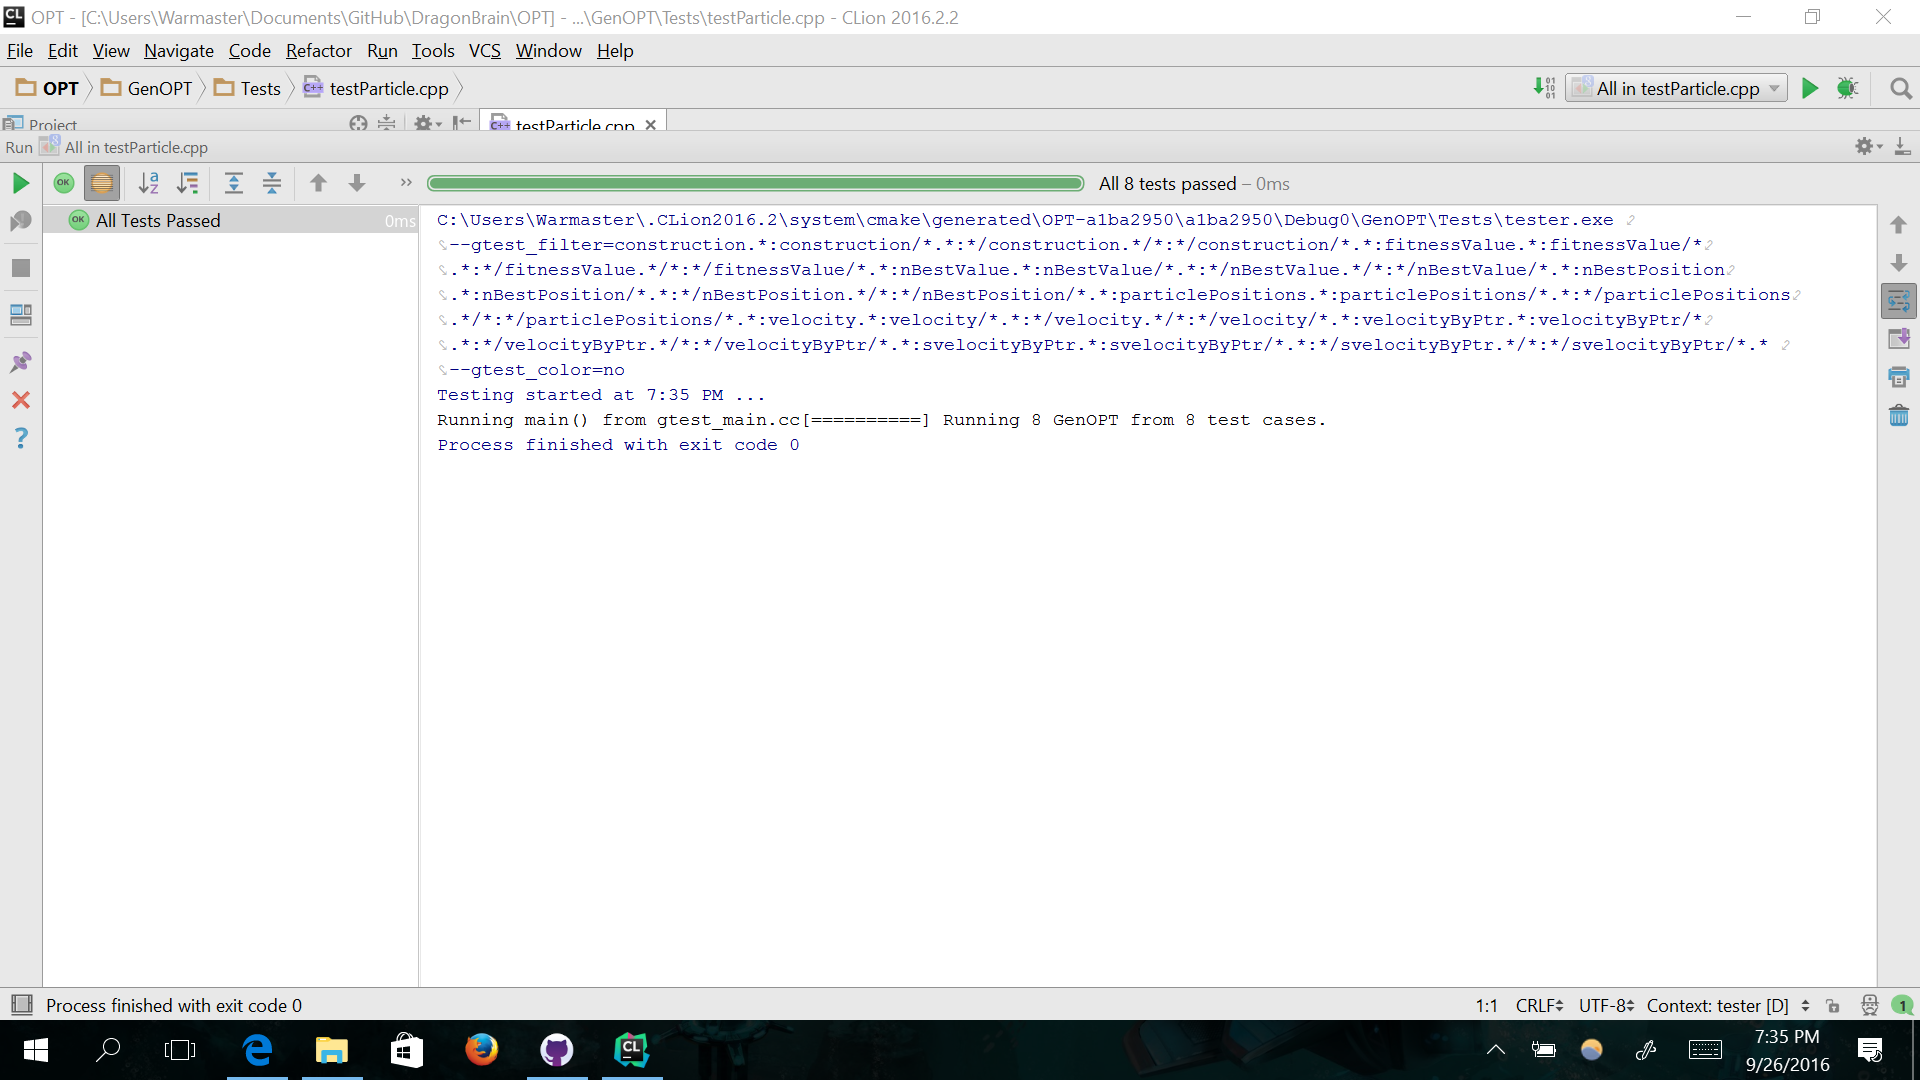
\includegraphics[scale=0.2]{Particle.png}
\caption{Example Unit Test Performed}
\end{figure}

\begin{figure}[h]
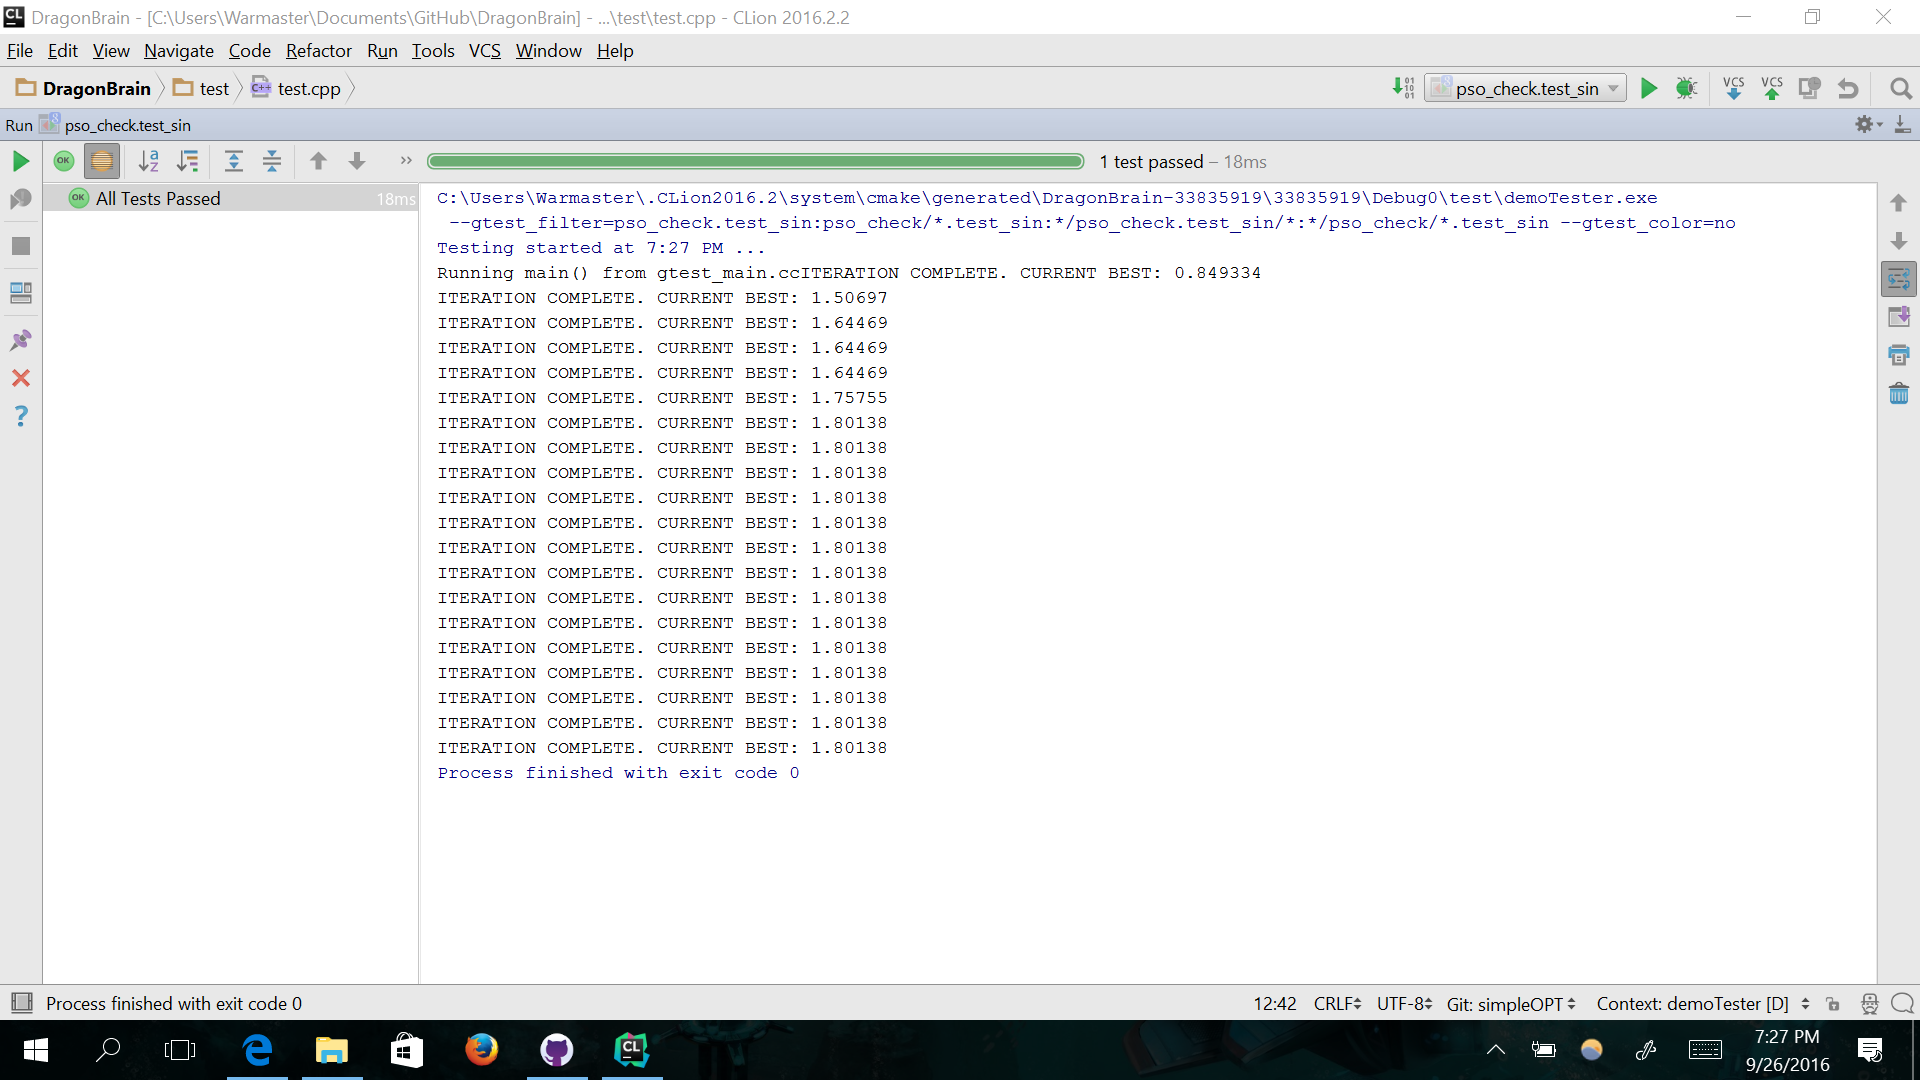
\includegraphics[scale=0.2]{psoTest.png}
\caption{Example Unit Test Performed}
\end{figure}
\begin{figure}[h]
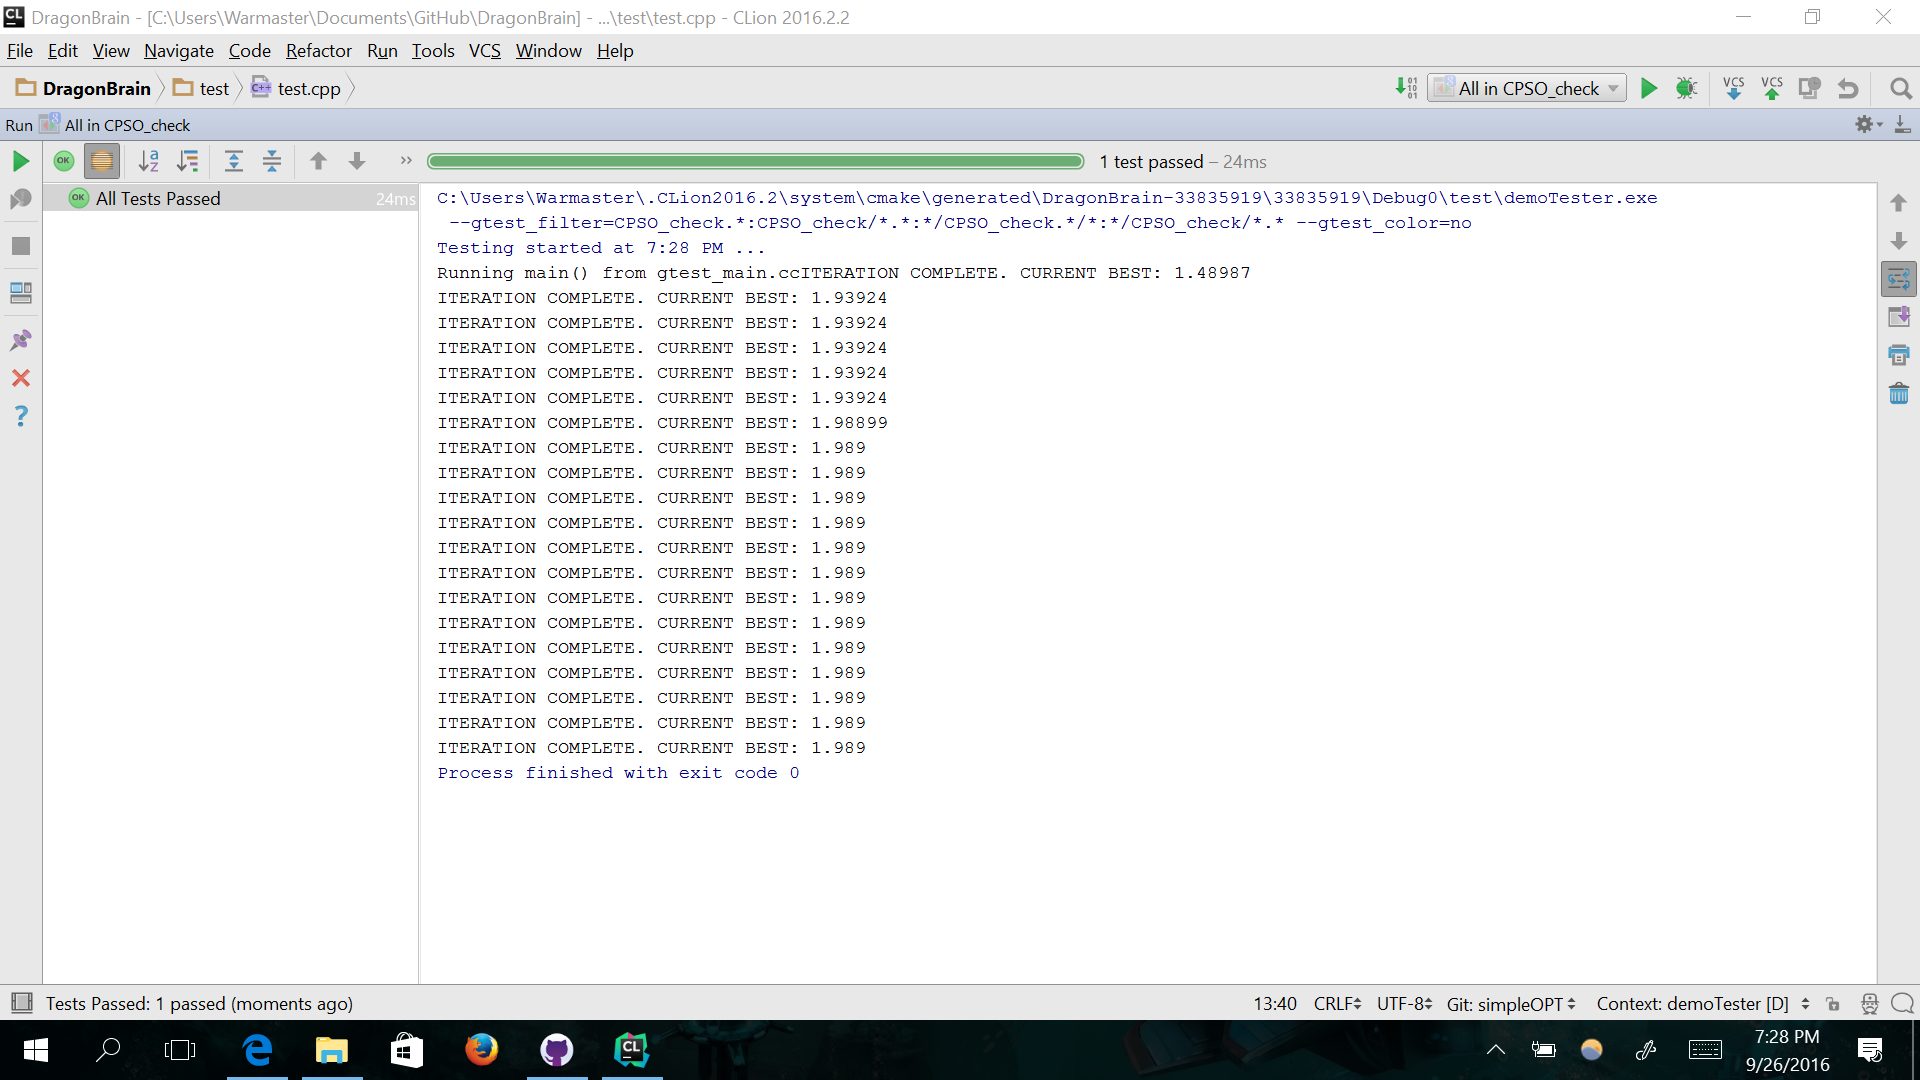
\includegraphics[scale=0.2]{cPSOcheck.png}
\caption{Example Unit Test Performed}
\end{figure}
\begin{figure}[h]
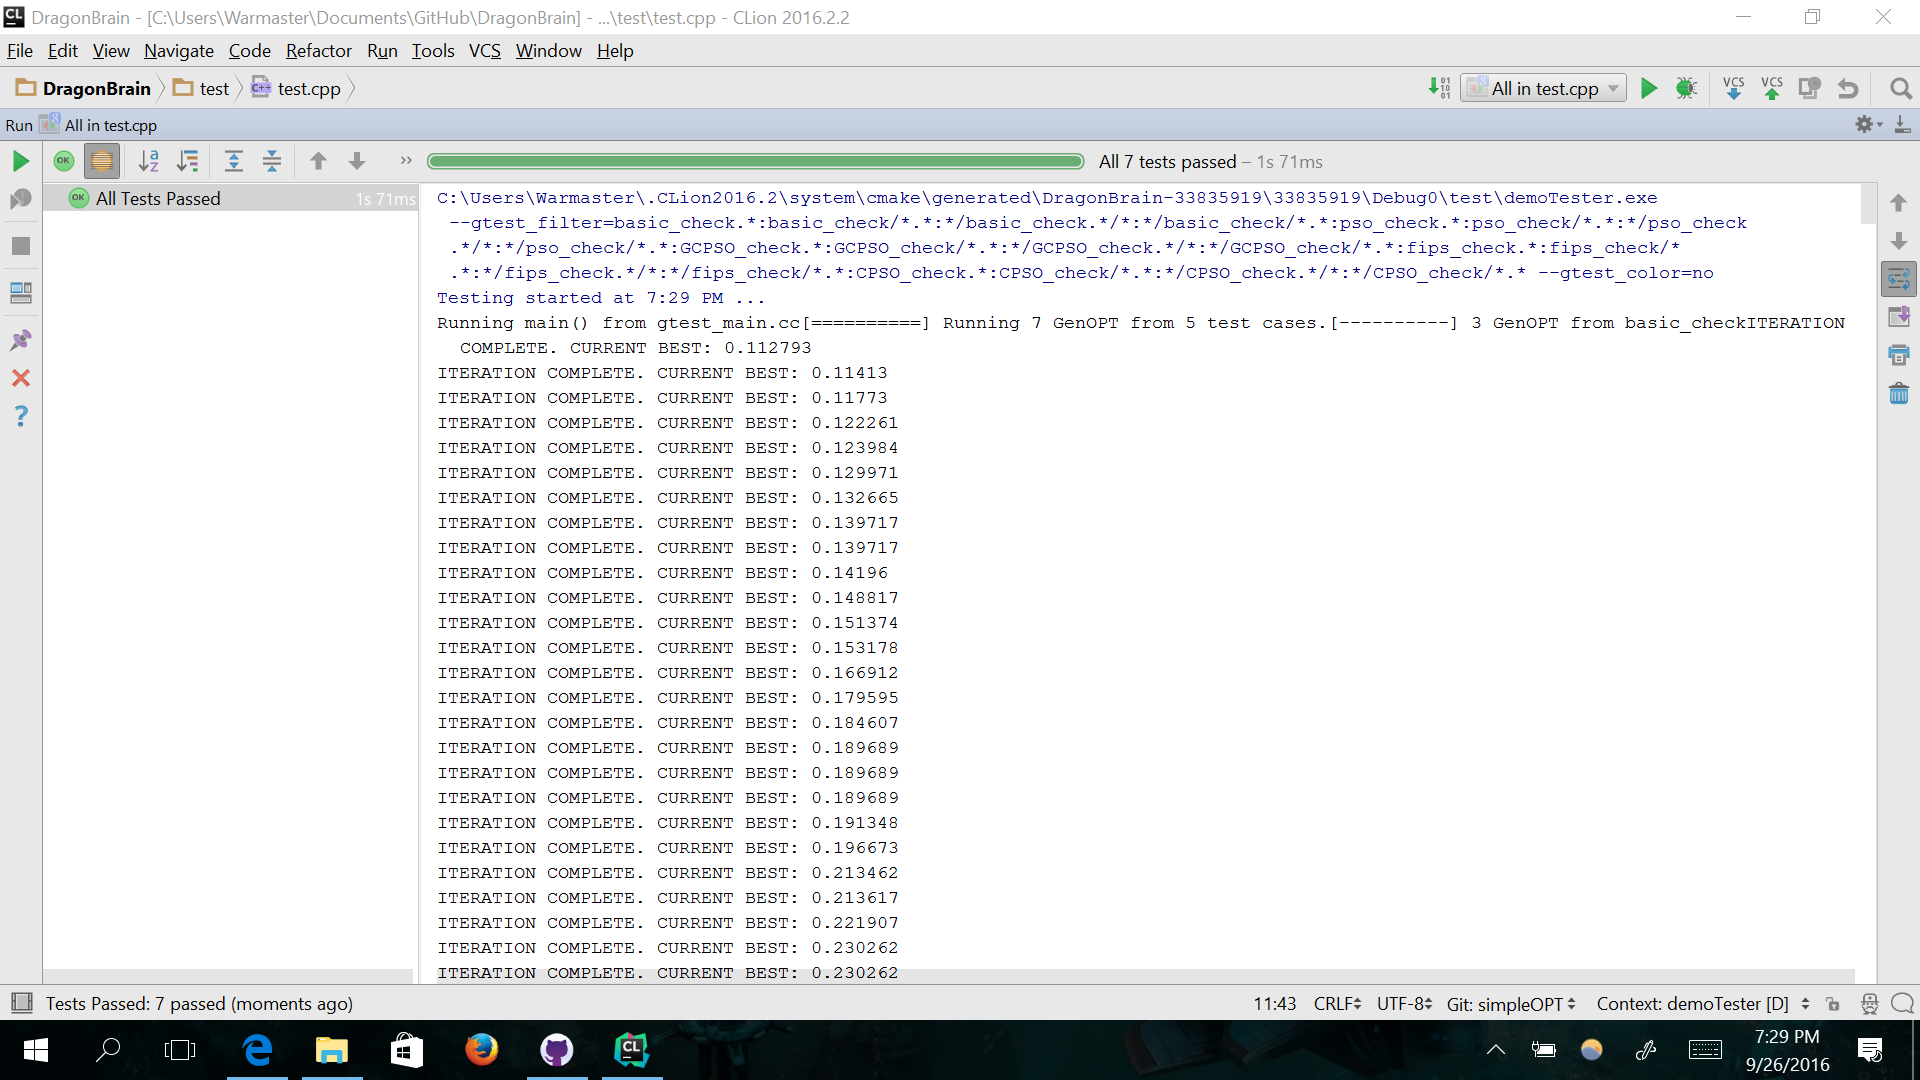
\includegraphics[scale=0.2]{hillClimbTest.png}
\caption{Example Unit Test Performed}
\end{figure}

\end{document}

